\subsection{Evaluation Settings}
\myparagraph{Testbed}
The evaluation was conducted on a custom four-wheeled robot (Fig~\ref{fig:robot}), and a custom air-ground robot(Fig~\ref{fig:agr}).
They are equipped with a Jetson Xavier NX~\cite{jetsonnx} 8G onboard computer that is capable of AI model inference with local computation resources. 
The system runs Ubuntu 20.04 with ROS Noetic and a dual-band USB network card (MediaTek MT76x2U) for wireless connectivity. 
The Jetson Xavier NX interfaces with a Leishen N10P LiDAR, ORBBEC Astra depth camera, and an STM32F407VET6 controller via USB serial ports. 
Both LiDAR and depth cameras facilitate environmental perception, enabling autonomous navigation, obstacle avoidance, and SLAM mapping. 
The GPU server is a PC equipped with an Intel(R) i5 12400f CPU @ 4.40GHz and an NVIDIA GeForce GTX 2080 Ti 11GB GPU, connected to our robot via Wi-Fi 6 over 80MHz channel at 5GHz frequency in our experiments.

Tab.~\ref{tab:energydefault} presents the overall on-board energy consumption (excluding motor energy consumption for robot movement) of the robot in various states: inference (model inference with full GPU utilization, including CPU and GPU energy consumption), transmission (communication with the GPU server, including wireless network card energy consumption), and standby (robot has no tasks to execute).
Notice that different models, due to varying numbers of parameters, exhibit distinct GPU utilization rates and power consumption during inference. 

\begin{table}[!t]
    \centering
    \begin{tabular}{|c|c|c|c|}
    \hline
            & inference & transmission & standby \\ \hline
    Power (W) &     13.35        &       4.25        &    4.04   \\ \hline
    \end{tabular}
    \caption{Power consumption (Watt) of our robot in different states.}
    \label{tab:energydefault}
    \end{table}

\myparagraph{Workload}
We evaluated two typical real-world robotic applications on our testbed: Kapao, a real-time people-tracking application on our four-wheeled robot (Fig~\ref{fig:kapao}), and AGRNav, an autonomous navigation application on our air-ground robot (Fig~\ref{fig:agrnav}). 
These applications feature different model input and output size patterns: Kapao takes RGB images as input and outputs key points of small data volume. In contrast, AGRNav takes point clouds as input and outputs predicted point clouds and semantics of similar data volume as input, implying that AGRNav needs to transmit more data during distributed inference. 
And we have verified several models common to mobile devices on a larger scale to further corroborate our observations and findings: DenseNet~\cite{huang2018densely}, VGGNet~\cite{simonyan2015deep}, ConvNeXt~\cite{woo2023convnext}, RegNet~\cite{xu2022regnet}.
% The models' running statistics are listed in Tab.~\ref{tab:all_app}.  

\myparagraph{Experiment Environments}
We evaluated two real-world environments: indoors (robots move in our laboratory with desks and separators interfering with wireless signals) and outdoors (robots move in our campus garden with trees and bushes interfering with wireless signals, resulting in lower bandwidth). 
The corresponding bandwidths between the robot and the GPU server in indoors and outdoors scenarios are shown in Fig.~\ref{fig:bandwidth}.

\myparagraph{Baselines}
We selected two SOTA inference acceleration methods as baselines: DSCCS ~\cite{liang2023dnn}, aimed at accelerating inference, and Hybrid-Parallel ~\cite{sun2024hybridparallel} (referred to as HP), that parallelizes local computation and offloading to further acceleratio inference. 
We also combined DSCCS with our cache mechanism (referred to as DSCCS-C) to present another perspective about CacheInf's performance gain.

The evaluation questions are as follows:
\begin{itemize}
    \item RQ1: How much does CacheInf benefit real-world robotic applications by reducing inference time and energy consumption?
    \item RQ2: How does CacheInf perform on more models common to mobile devices?
    \item RQ3: How is the above gain achieved in CacheInf?
    \item RQ4: What are the limitations and potentials of CacheInf?
\end{itemize}

\begin{figure}[!t]
    \centering
    \subfloat[Targeted people]{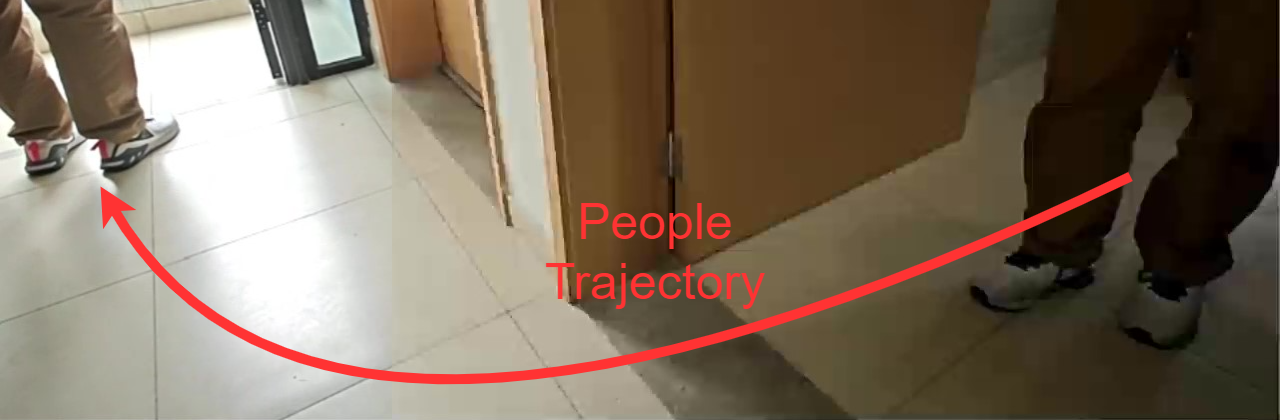
\includegraphics[width=0.48\linewidth]{fig/people.drawio.png}}
    \hfil
    \subfloat[Robot moving trajectory]{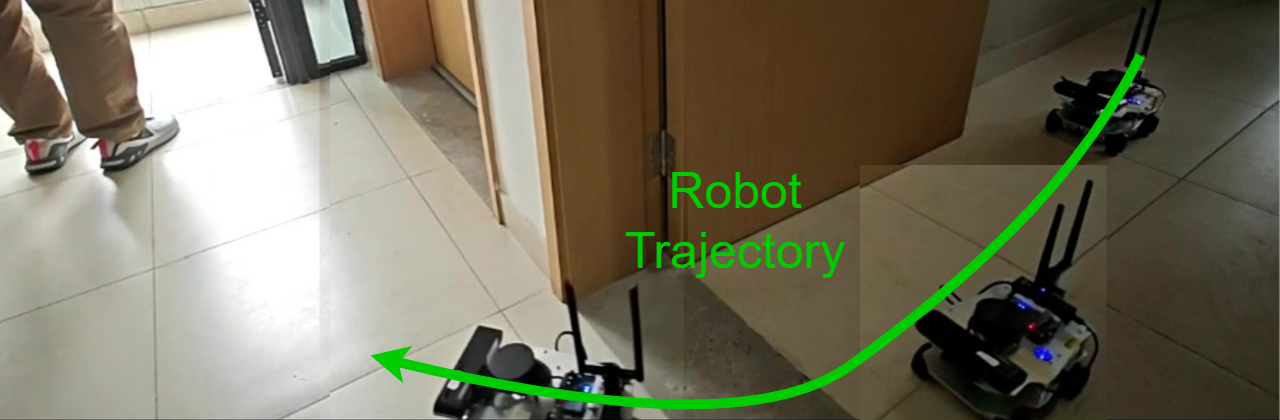
\includegraphics[width=0.48\linewidth]{fig/robot.drawio.png}}
    \caption{A real-time people-tracking robotic application on our robot based on a well-known human pose estimation ML model, Kapao~\cite{kapao}.}
    \label{fig:kapao}
\end{figure}

\begin{figure}[!t]
    \centering
    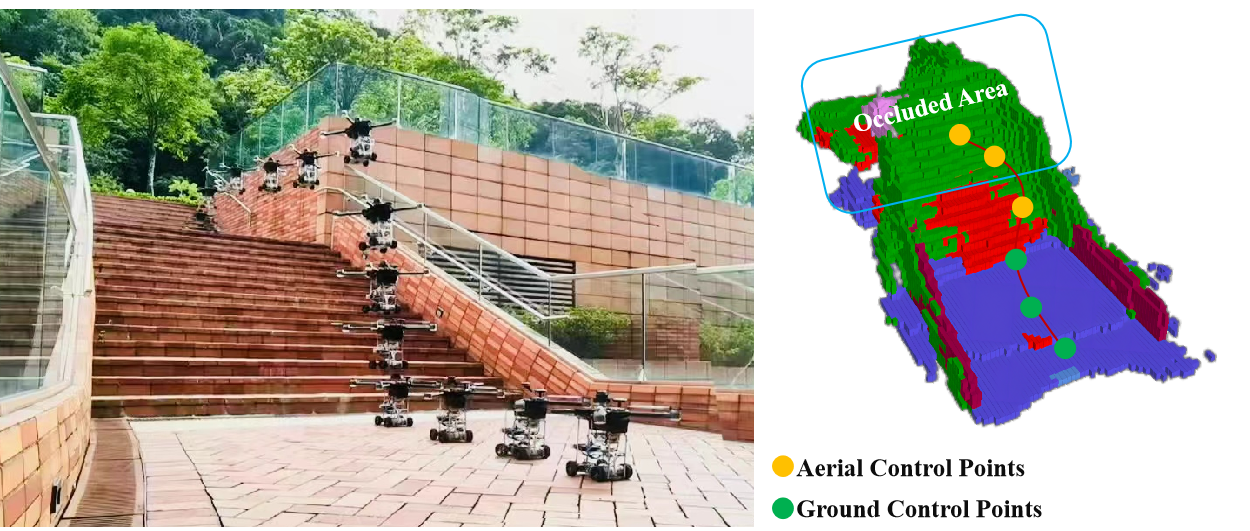
\includegraphics[width=0.98\linewidth]{fig/agrnav.png}
    \caption{By predicting occlusions in advance, AGRNav~\cite{agrnav} gains an accurate perception of the environment and avoids collisions, resulting in efficient and energy-saving paths.}
    \label{fig:agrnav}
\end{figure}


\subsection{End-to-End Performance on Real-World Applications}

\myparagraph{Inference Time}
\begin{table*}[htb]
    \centering

\begin{tabular}{ccc|c|c|c|c|c|c}
\toprule
Model(number & Local compu- & \multirow[c]{2}{*}{System} & \multicolumn{2}{|c|}{Transmission time/s} & \multicolumn{2}{|c|}{Inference time/s} & \multicolumn{2}{c}{Percentage(\%)} \\
of parameters)& tation time/s &  & indoors & outdoors & indoors & outdoors & indoors & outdoors \\
\midrule
\multirow[c]{4}{*}{kapao(77M)} & \multirow[c]{4}{*}{1.01($\pm$0.03)} & DSCCS & 0.21($\pm$0.1) & 0.24($\pm$0.12) & 0.36($\pm$0.2) & 0.40($\pm$0.17) & 58.33 & 60.21 \\
 &  & DSCCS-C & 0.18($\pm$0.14) & 0.22($\pm$0.12) & 0.33($\pm$0.25) & 0.37($\pm$0.18) & 66.67 & 67.57 \\
 &  & Hybrid-Parallel & 0.24($\pm$0.15) & 0.28($\pm$0.13) & 0.31($\pm$0.14) & 0.34($\pm$0.12) & 77.42 & 82.35 \\
 &  & CacheInf & 0.16($\pm$0.13) & 0.21($\pm$0.18) & 0.20($\pm$0.16) & 0.24($\pm$0.20) & 80.09 & 87.56 \\
\cline{1-9} \cline{2-9}
\multirow[c]{4}{*}{agrnav(0.84M)} & \multirow[c]{4}{*}{0.60($\pm$0.04)} & DSCCS & 0.10($\pm$0.05) & 0.15($\pm$0.05) & 0.41($\pm$0.11) & 0.47($\pm$0.12) & 24.39 & 31.91\\
 &  & DSCCS-C & 0.13($\pm$0.07) & 0.16($\pm$0.06) & 0.38($\pm$0.10) & 0.43($\pm$0.13) & 34.21 & 37.21\\
 &  & Hybrid-Parallel & 0.24($\pm$0.08) & 0.26($\pm$0.07) & 0.30($\pm$0.09) & 0.33($\pm$0.07) & 78.65 & 79.47 \\
 &  & CacheInf & 0.18($\pm$0.08) & 0.20($\pm$0.08) & 0.21($\pm$0.16) & 0.25($\pm$0.18) & 86.71 & 80.01 \\
\cline{1-9} \cline{2-9}
\bottomrule
\end{tabular}


    \caption{Average transmission time, inference time, percentage that transmission time accounts for of the total inference time and their standard deviation ($\pm n$) of Kapao and AGRNav in different environments with different systems. ``Local computation'' refers to inference the entire model locally on the robot.}
    \label{tab:e2e_time}
\end{table*}

\myparagraph{Energy Consumption}
\begin{table*}[htb]
\centering
\begin{tabular}{cc|c|c|c|c}
\toprule
 Model(number & \multirow[c]{2}{*}{System} & \multicolumn{2}{|c|}{Power consumption(W)} & \multicolumn{2}{|c}{Energy consumption(J) per inference} \\
 of parameters)&  & indoors & outdoors & indoors & outdoors \\
\midrule
\midrule
\multirow[c]{5}{*}{kapao(77M)} & Local & 10.61($\pm$0.49) & 10.61($\pm$0.49) & 9.79($\pm$0.03) & 9.79($\pm$0.03) \\
 & DSCCS & 6.38($\pm$2.21) & 6.63($\pm$2.38) & 2.30($\pm$0.55) & 2.65($\pm$0.55) \\
 & DSCCS-C & 6.30($\pm$2.15) & 6.53($\pm$2.12) & 2.08($\pm$0.50) & 2.42($\pm$0.53) \\
 & HP & 7.05($\pm$1.63) & 6.94($\pm$0.98) & 2.19($\pm$0.62) & 2.35($\pm$0.42) \\
 & CacheInf & 7.53($\pm$1.62) & 7.30($\pm$0.96) & 1.51($\pm$0.60) & 2.75($\pm$0.41) \\
\cline{1-6}
\multirow[c]{5}{*}{agrnav(0.84M)} & Local & 8.11($\pm$0.25) & 8.11($\pm$0.25) & 4.86($\pm$0.01) & 4.86($\pm$0.01) \\
 & DSCCS & 6.21($\pm$1.50) & 7.29($\pm$1.55) & 2.55($\pm$0.19) & 3.43($\pm$0.18) \\
 & DSCCS-C & 6.17($\pm$1.56) & 7.00($\pm$1.43) & 2.34($\pm$0.20) & 3.01($\pm$0.20) \\
 & HP & 7.52($\pm$0.51) & 8.04($\pm$0.45) & 2.26($\pm$0.15) & 2.63($\pm$0.15) \\
 & CacheInf & 7.83($\pm$0.57) & 8.23($\pm$0.56) & 1.64($\pm$0.17) & 2.06($\pm$0.16) \\
\cline{1-6}
\bottomrule
\end{tabular}

    \caption{The power consumption against time (Watt) and energy consumption per inference (Joule) with standard deviation ($\pm n$) of Kapao and AGRNav different environments with different systems. ``Local'' represents ``Local computation''.}
    \label{tab:e2e_power}
\end{table*}

\subsection{Performance on Other Common Models}

\begin{table*}[htb]

    \centering
\begin{tabular}{ccc|c|c|c|c|c|c}
\toprule
 Model(number&  Local compu- & \multirow[c]{2}{*}{System} & \multicolumn{2}{|c|}{Transmission time/ms} & \multicolumn{2}{|c|}{Inference time/ms} & \multicolumn{2}{c}{Percentage(\%)} \\
 of parameters) & taion time/ms &  & indoors & outdoors & indoors & outdoors & indoors & outdoors \\
\midrule
\multirow[c]{4}{*}{DenseNet121(7M)} & \multirow[c]{4}{*}{74.5($\pm$18.7)} & DSCCS & 16.2($\pm$40.9) & 20.8($\pm$51.9) & 81.4($\pm$27.2) & 86.6($\pm$27.7) & 19.95 & 24.07 \\
 &  & DSCCS-C & 20.4($\pm$43.5) & 25.8($\pm$56.9) & 85.5($\pm$27.9) & 89.6($\pm$29.3) & 23.86 & 28.80 \\
 &  & HP & 53.4($\pm$34.5) & 52.9($\pm$23.9) & 74.5($\pm$85.7) & 55.1($\pm$15.6) & 71.70 & 96.05 \\
 &  & CacheInf & 56.3($\pm$37.5) & 57.5($\pm$43.5) & 76.3($\pm$90.6) & 78.1($\pm$33.6) & 73.79 & 73.62 \\
\cline{1-9} \cline{2-9}
\multirow[c]{4}{*}{RegNet(54M)} & \multirow[c]{4}{*}{175.0($\pm$23.6)} & DSCCS & 47.6($\pm$47.8) & 60.5($\pm$54.0) & 77.8($\pm$39.3) & 86.2($\pm$37.9) & 61.22 & 70.22 \\
 &  & DSCCS-C & 50.7($\pm$49.8) & 62.5($\pm$53.6) & 70.8($\pm$33.3) & 79.5($\pm$39.2) & 71.61 & 78.61 \\
 &  & HP & 49.6($\pm$21.7) & 59.9($\pm$23.4) & 55.0($\pm$24.8) & 64.2($\pm$25.2) & 90.18 & 93.34 \\
 &  & CacheInf & 44.2($\pm$27.7) & 48.5($\pm$25.3) & 45.3($\pm$35.0) & 49.2($\pm$37.2) & 97.57 & 98.58 \\
\cline{1-9} \cline{2-9}
\multirow[c]{4}{*}{ConvNeXt(88M)} & \multirow[c]{4}{*}{160.2($\pm$21.0)} & DSCCS & 46.9($\pm$43.1) & 56.7($\pm$52.1) & 72.4($\pm$35.7) & 84.7($\pm$36.3) & 64.78 & 66.95 \\
 &  & DSCCS-C & 48.0($\pm$45.0) & 53.2($\pm$50.1) & 56.8($\pm$28.1) & 70.8($\pm$39.0) & 84.51 & 75.14 \\
 &  & HP & 50.4($\pm$32.2) & 61.9($\pm$34.8) & 53.9($\pm$26.2) & 65.7($\pm$27.7) & 93.51 & 94.23 \\
 &  & CacheInf & 40.7($\pm$40.0) & 50.7($\pm$40.3) & 46.7($\pm$35.4) & 56.8($\pm$45.0) & 87.15 & 89.26 \\
\cline{1-9} \cline{2-9}
\multirow[c]{4}{*}{VGG19(143M)} & \multirow[c]{4}{*}{118.0($\pm$18.9)} & DSCCS & 38.9($\pm$47.1) & 41.6($\pm$53.8) & 65.2($\pm$28.1) & 75.5($\pm$27.1) & 59.75 & 55.09 \\
 &  & DSCCS-C & 42.7($\pm$30.2) & 52.0($\pm$50.3) & 53.2($\pm$33.0) & 60.3($\pm$30.9) & 80.26 & 86.24 \\
 &  & HP & 44.8($\pm$20.9) & 51.5($\pm$15.0) & 47.6($\pm$18.1) & 53.6($\pm$14.7) & 94.15 & 96.07 \\
 &  & CacheInf & 37.8($\pm$31.2) & 43.5($\pm$13.2) & 41.1($\pm$20.3) & 46.6($\pm$12.8) & 94.26 & 93.34 \\
\cline{1-9} \cline{2-9}
\multirow[c]{4}{*}{ConvNeXt(197M)} & \multirow[c]{4}{*}{316.7($\pm$31.0)} & DSCCS & 56.0($\pm$36.1) & 67.0($\pm$37.6) & 79.2($\pm$35.9) & 90.6($\pm$35.4) & 70.72 & 73.98 \\
 &  & DSCCS-C & 56.0($\pm$39.0) & 63.0($\pm$30.2) & 64.7($\pm$40.2) & 68.6($\pm$35.0) & 86.55 & 91.84 \\
 &  & HP & 56.4($\pm$34.7) & 66.5($\pm$33.7) & 59.7($\pm$26.6) & 68.0($\pm$26.6) & 94.43 & 97.88 \\
 &  & CacheInf & 40.4($\pm$37.8) & 46.9($\pm$40.0) & 44.7($\pm$33.3) & 49.0($\pm$30.8) & 90.38 & 95.71 \\
\cline{1-9} \cline{2-9}
\bottomrule
\end{tabular}


    \caption{Average transmission time, inference time, percentage that transmission time accounts for of the total inference time and their standard deviation ($\pm n$) of common AI models in different environments with different systems. }
    \label{tab:torchvision_time}
\end{table*}

\begin{table*}[htb]

\centering
\begin{tabular}{cc|c|c|c|c}
\toprule
Model(number & \multirow[c]{2}{*}{System} & \multicolumn{2}{|c|}{Power consumption(W)} & \multicolumn{2}{|c}{Energy consumption(J) per inference} \\
of parameters)&  & indoors & outdoors & indoors & outdoors \\
\midrule
\multirow[c]{5}{*}{DenseNet121(7M)} & Local & 8.2($\pm$0.27) & 8.2($\pm$0.27) & 0.46($\pm$0.04) & 0.46($\pm$0.04) \\
 & DSCCS & 6.91($\pm$0.45) & 6.86($\pm$0.46) & 0.56($\pm$0.04) & 0.59($\pm$0.04) \\
 & DSCCS-C & 7.01($\pm$0.43) & 6.96($\pm$0.43) & 0.60($\pm$0.07) & 0.52($\pm$0.06) \\
 & HP & 5.36($\pm$0.79) & 5.79($\pm$0.24) & 0.4($\pm$0.06) & 0.32($\pm$0.01) \\
 & CacheInf & 6.01($\pm$0.92) & 6.31($\pm$0.56) & 0.46($\pm$0.12) & 0.49($\pm$0.01) \\
\cline{1-6}
\multirow[c]{5}{*}{RegNet(54M)} & Local & 9.0($\pm$0.3) & 9.0($\pm$0.3) & 1.37($\pm$0.02) & 1.37($\pm$0.02) \\
& DSCCS & 5.84($\pm$1.79) & 5.36($\pm$1.34) & 0.45($\pm$0.14) & 0.46($\pm$0.12) \\
 & DSCCS-C & 6.04($\pm$1.88) & 5.96($\pm$1.45) & 0.43($\pm$0.16) & 0.47($\pm$0.19) \\
 & HP & 5.24($\pm$1.43) & 5.28($\pm$1.52) & 0.29($\pm$0.08) & 0.34($\pm$0.1) \\
 & CacheInf & 5.20($\pm$1.51) & 5.43($\pm$1.77) & 0.24($\pm$0.08) & 0.327($\pm$0.09) \\
\cline{1-6}
\multirow[c]{5}{*}{ConvNeXt(88M)} & Local & 9.7($\pm$0.34) & 9.7($\pm$0.34) & 1.34($\pm$0.02) & 1.34($\pm$0.02) \\
& DSCCS & 6.01($\pm$0.27) & 5.71($\pm$1.56) & 0.43($\pm$0.05) & 0.48($\pm$0.13) \\
& DSCCS-C & 6.20($\pm$0.33) & 5.91($\pm$0.21) & 0.35($\pm$0.17) & 0.42($\pm$0.25) \\
 & HP & 6.68($\pm$1.23) & 6.68($\pm$1.21) & 0.36($\pm$0.07) & 0.44($\pm$0.08) \\
 & CacheInf & 6.70($\pm$0.55) & 6.63($\pm$0.26) & 0.31($\pm$0.07) & 0.38($\pm$0.08) \\
\cline{1-6}
\multirow[c]{5}{*}{VGG19(143M)} & Local & 9.78($\pm$0.34) & 9.78($\pm$0.34) & 0.95($\pm$0.02) & 0.95($\pm$0.02) \\
& DSCCS & 6.58($\pm$2.14) & 6.93($\pm$2.35) & 0.43($\pm$0.14) & 0.52($\pm$0.18) \\
 & DSCCS-C & 6.82($\pm$2.10) & 7.23($\pm$2.45) & 0.36($\pm$0.18) & 0.43($\pm$0.30) \\
 & HP & 6.51($\pm$1.74) & 7.32($\pm$1.52) & 0.31($\pm$0.08) & 0.39($\pm$0.08) \\
 & CacheInf & 6.70($\pm$1.88) & 7.22($\pm$1.36) & 0.27($\pm$0.10) & 0.34($\pm$0.09) \\
\cline{1-6}
\multirow[c]{5}{*}{ConvNeXt(197M)} & Local & 10.72($\pm$0.38) & 10.72($\pm$0.38) & 3.12($\pm$0.03) & 3.12($\pm$0.03) \\
& DSCCS & 5.06($\pm$0.31) & 5.02($\pm$0.37) & 0.4($\pm$0.02) & 0.45($\pm$0.03) \\
 & DSCCS-C & 4.86($\pm$0.44) & 4.99($\pm$0.39) & 0.31($\pm$0.05) & 0.34($\pm$0.09) \\
 & HP & 4.57($\pm$0.23) & 4.54($\pm$0.25) & 0.27($\pm$0.01) & 0.31($\pm$0.02) \\
 & CacheInf & 5.26($\pm$0.40) & 5.39($\pm$0.27) & 0.24($\pm$0.05) & 0.26($\pm$0.04) \\
\cline{1-6}
\bottomrule
\end{tabular}
    \caption{The power consumption against time (Watt) and energy consumption per inference (Joule) with standard deviation ($\pm n$) of common AI models in different environments with different systems. ``Local'' represents ``Local computation''.}
    \label{tab:torchvision_power}
\end{table*}

\subsection{Breakdown}

\subsection{Discussion}